\documentclass[12pt, letterpaper]{article}
\usepackage[top=2.5cm, bottom=2.5cm, left=3cm, right=2.5cm]{geometry}
\usepackage[utf8]{inputenc}
\usepackage[T1]{fontenc}
\usepackage{lmodern}
\usepackage{amsmath, amssymb}
\usepackage{booktabs}
\usepackage{tabularx}
\usepackage{longtable}
\usepackage{array}
\usepackage{multirow}
\usepackage{xcolor}
\usepackage{graphicx}
\usepackage{float}
\usepackage{listings}
\usepackage[most, breakable]{tcolorbox}
\usepackage{enumitem}
\usepackage{fancyhdr}
\usepackage{titlesec}
\usepackage{setspace}
\usepackage{microtype}
\usepackage[hidelinks]{hyperref}
\usepackage{parskip}
\usepackage{tikz}
\usepackage{pgfplots}
\pgfplotsset{compat=1.15}
\usepackage{amsmath}

% Colours
\definecolor{econblue}{RGB}{31,78,121}
\definecolor{researchgreen}{RGB}{21,101,45}
\definecolor{exampleorange}{RGB}{180,80,20}
\definecolor{lightgray}{RGB}{245,245,245}
\definecolor{boxblue}{RGB}{220,235,248}

% Section headings
\titleformat{\section}{\large\bfseries\color{econblue}}{\thesection}{1em}{}%
  [\vspace{-4pt}\rule{\linewidth}{0.4pt}]
\titleformat{\subsection}{\normalsize\bfseries\color{econblue}}{\thesubsection}{1em}{}
\titleformat{\subsubsection}{\normalsize\bfseries}{\thesubsubsection}{1em}{}

% Page style
\pagestyle{fancy}
\fancyhf{}
\fancyhead[L]{\small\itshape ECON 230 --- Introduction to Behavioural Economics}
\fancyhead[R]{\small\itshape Chapter 7: Strategic Behaviour}
\fancyfoot[C]{\small\thepage}
\renewcommand{\headrulewidth}{0.4pt}
\setlength{\headheight}{14pt}

% tcolorbox styles
\tcbuselibrary{breakable, skins, listings}

\newtcolorbox{researchbox}{
  enhanced, breakable,
  colback=researchgreen!6, colframe=researchgreen!55,
  title=\textbf{Research Study},
  fonttitle=\bfseries\small,
  attach boxed title to top left={yshift=-2mm, xshift=6mm},
  boxed title style={colback=researchgreen!55, colframe=researchgreen!55},
  before upper={\setlength{\parskip}{4pt}}
}

\newtcolorbox{examplebox}[1]{
  enhanced, breakable,
  colback=exampleorange!6, colframe=exampleorange!45,
  title=\textbf{#1}, fonttitle=\bfseries\small
}

\newtcolorbox{keybox}{
  enhanced, colback=boxblue, colframe=econblue!70,
  fontupper=\small
}

% ASCII figure style
\lstset{
  basicstyle=\scriptsize\ttfamily,
  breaklines=false,
  keepspaces=true,
  columns=flexible,
  frame=single,
  backgroundcolor=\color{lightgray},
  xleftmargin=4pt, xrightmargin=4pt,
  aboveskip=6pt, belowskip=6pt
}

% Lists
\setlist[itemize]{leftmargin=1.5em, itemsep=2pt, topsep=4pt}
\setlist[enumerate]{leftmargin=1.5em, itemsep=2pt, topsep=4pt}
\onehalfspacing

\newcolumntype{Y}{>{\raggedright\arraybackslash}X}

\begin{document}

\begin{titlepage}
\centering\vspace*{3cm}
{\Large\bfseries\color{econblue} ECON 230 --- Introduction to Behavioural Economics\\[1em]}
{\large\bfseries Course Textbook\\[2em]}
{\LARGE\bfseries\color{econblue} Chapter 7\\[0.5em]}
{\Large\bfseries Strategic Behaviour --- Behavioural Game Theory\\[2em]}
\vfill
{\normalsize University of Northern British Columbia\\
Instructor: Prof.\ Muhebullah Karimzada\\
Term: Winter 2027}
\end{titlepage}
\tableofcontents
\newpage





\section*{Chapter Overview}
\addcontentsline{toc}{section}{Chapter Overview}


Classical game theory is one of the most elegant and powerful tools in all of economics. It provides a rigorous framework for analysing situations in which the outcome of one agent's decision depends on what other agents decide --- from firms competing for market share, to countries negotiating treaties, to drivers navigating intersections, to individuals bidding at auction. Its centrepiece concept, Nash equilibrium, offers a clean prediction: in a Nash equilibrium, no player can improve their outcome by unilaterally changing their strategy. It is the natural resting point of strategic interaction among fully rational agents.

The difficulty is that reaching Nash equilibrium typically requires not just individual rationality but an extraordinarily demanding chain of mutual reasoning. Players must be rational, must know that others are rational, must know that others know that they are rational, and so on --- to infinite depth. This requirement, called \textbf{Common Knowledge of Rationality (CKR)}, is almost certainly violated in practice. Real people reason about others' strategies to limited depths, make mistakes, have different beliefs about others' beliefs, and bring all the cognitive limitations documented in Chapters 1 through 3 into their strategic interactions.

\textbf{Behavioural game theory} is the project of building more realistic models of strategic reasoning --- models that relax the CKR requirement, incorporate bounded rationality and social preferences, and make predictions that fit the data better than classical game theory. This chapter introduces its central tools.

We begin by making precise what CKR requires and why it is implausible. We then study the \textbf{level-k model} of iterated strategic reasoning, which replaces infinite recursion with a finite reasoning depth and predicts that most people reason only one or two steps. We analyse the \textbf{Keynesian beauty contest} --- the canonical game for studying level-k reasoning --- and show how the model predicts the clustering of guesses around 33 rather than the Nash equilibrium prediction of 0.

We examine the \textbf{prisoner's dilemma} --- perhaps the most famous game in all of social science --- and the conditions under which cooperation can be sustained in its repeated version through the folk theorem and strategies like \textbf{Tit-for-Tat}. We study the \textbf{centipede game} as a test of backward induction, where theory predicts immediate defection but experiment finds sustained cooperation. We introduce \textbf{Quantal Response Equilibrium} as a formal model of boundedly rational strategic choice. We close with applications to auctions and the \textbf{winner's curse}, oligopoly, and the strategic implications for business and policy.

\medskip


\section*{Learning Objectives}
\addcontentsline{toc}{section}{Learning Objectives}


After studying this chapter, students should be able to:

\begin{enumerate}
\item \textbf{Define} Nash equilibrium and explain the Common Knowledge of Rationality requirement it imposes on strategic reasoning.
\item \textbf{Identify} the sources of Nash equilibrium failure in real strategic settings, including limited reasoning depth, social preferences, and bounded rationality.
\item \textbf{Define} the level-k model, describe the reasoning process at each level from L0 to L3, and explain why most empirical evidence places most people at L1--L2.
\item \textbf{Apply} level-k reasoning to the Keynesian beauty contest game, deriving the prediction at each level and interpreting real experimental data.
\item \textbf{Analyse} the prisoner's dilemma --- its payoff structure, its Nash equilibrium, the efficiency cost of that equilibrium, and real-world applications.
\item \textbf{Explain} the folk theorem for infinitely repeated games and describe why repetition enables cooperation that is impossible in one-shot games.
\item \textbf{Describe} Tit-for-Tat and explain its four properties that make it an effective cooperation strategy.
\item \textbf{Describe} the centipede game, derive the backward induction prediction, and explain why empirical results diverge from it.
\item \textbf{Define} Quantal Response Equilibrium, interpret its parameter $\lambda$, and explain how it nests Nash equilibrium as a special case.
\item \textbf{Apply} behavioural game theory to auctions (the winner's curse), oligopoly (tacit collusion), and corporate mergers and acquisitions.
\end{enumerate}

\medskip


\section*{Introduction: The Limits of Perfect Strategic Reasoning}
\addcontentsline{toc}{section}{Introduction: The Limits of Perfect Strategic Reasoning}


Before reading any further, write down a number between 0 and 100. The winner of the game is the person whose number is closest to \textbf{two-thirds of the average} number chosen by all players.

Take a moment. Write it down.

This game --- known as the Keynesian beauty contest or the $p$-beauty contest --- is one of the most illuminating experiments in behavioural economics. Its Nash equilibrium is unambiguous: if everyone reasons correctly and knows everyone else reasons correctly, all players should choose 0. (We will derive this shortly.) Yet in experiments conducted with thousands of participants --- from undergraduate students to experienced economists and financial professionals --- almost nobody chooses 0. Most people choose numbers between 20 and 40.

The gap between the Nash prediction and the data is not a failure of motivation or stakes. It reflects a genuine limitation in how far people carry their strategic reasoning --- how many steps of "if they think that I think that they think..." they can iterate before their reasoning stops. This chapter explains why this limitation is fundamental, models it formally, and explores its consequences for economic life.

\medskip


\section{Nash Equilibrium and What It Really Requires}



\subsection{The Concept}


A \textbf{Nash equilibrium} is a strategy profile $(s_1^*, s_2^*, \ldots, s_n^*)$ --- one strategy for each player --- such that no player can increase their payoff by unilaterally switching to a different strategy, given what all other players are doing.

Formally, for each player $i$:

$$u_i(s_i^*, s_{-i}^*) \geq u_i(s_i, s_{-i}^*) \quad \text{for all } s_i$$

where $s_{-i}^*$ denotes the strategies of all players other than $i$.

Nash equilibrium is the dominant solution concept in non-cooperative game theory, and for good reason: it is the only self-consistent prediction in the following sense. If a theorist predicts that players will use strategies $(s_1^*, \ldots, s_n^*)$ and each player believes the prediction, then no player has any incentive to deviate. The prediction is self-fulfilling. No other profile of strategies has this property.


\subsection{The CKR Requirement}


What does it take for players to actually arrive at a Nash equilibrium? The requirement is considerably more demanding than it might appear.

Consider a two-player game. For player 1 to play a Nash equilibrium strategy:
\begin{itemize}
\item Player 1 must be rational (choose the strategy that maximises their payoff given their beliefs about player 2).
\item Player 1 must \textit{know} what player 2 will do --- which requires knowing that player 2 is rational.
\item But to know that player 2 is rational, player 1 must know player 2's beliefs about player 1's strategy --- which requires knowing that player 2 knows player 1 is rational.
\item And to know that player 2 knows player 1 is rational, player 1 must know that player 2 knows that player 1 knows that player 2 is rational.
\item ... and so on, without end.
\end{itemize}

This infinite chain of mutual beliefs about beliefs about beliefs is called \textbf{Common Knowledge of Rationality (CKR)}. It is the epistemological requirement that everyone is rational, everyone knows that everyone is rational, everyone knows that everyone knows that everyone is rational, to any finite depth --- and that this is common knowledge.

CKR is an extraordinarily strong assumption. In everyday language, it means that every player in the game is a perfect reasoner, that every player knows every other player is a perfect reasoner, and that this is known to arbitrary depth by all players. A single player who might be irrational --- or who might make a strategic mistake --- is sufficient to invalidate CKR for all other players, who must now reason about the possibility of such a player.
\newpage

\textbf{Table 7.1: When Does CKR Fail?}


\begin{table}[H]
\centering
\small
\begin{tabularx}{\linewidth}{lYY}
\toprule
Failure Mode & Description & Example \\
\midrule
Limited reasoning depth & Players can only iterate $k$ steps of "I think that you think that I think..." & Most people stop at 1--2 steps \\
Bounded rationality & Players make computational errors or use heuristics & Cognitive limitations from Chapters 1--2 \\
Social preferences & Players have motivations beyond own payoff & Fairness, reciprocity (Chapter 6) \\
Unfamiliar game & Players have not played the game before & Novel strategic situations \\
Heterogeneous beliefs & Players disagree about others' rationality & Realistic in any population \\
\bottomrule
\end{tabularx}
\end{table}


CKR may be a reasonable approximation in highly competitive, well-functioning markets where agents have experience and strong financial incentives to reason correctly, and where selection has filtered out persistent reasoning errors. It is least reasonable in novel situations, among inexperienced players, and in games where the payoff structure makes the rational solution counterintuitive --- exactly the conditions of most economic and policy importance.

\medskip


\section{The Prisoner's Dilemma}


Before studying bounded rationality in strategic settings, we review the most famous game in social science, because it sets up all the subsequent discussion of cooperation, repeated interaction, and the limits of self-interest reasoning.


\subsection{The Game}


The \textbf{prisoner's dilemma} describes a situation in which two players each independently choose whether to \textbf{cooperate (C)} or \textbf{defect (D)}, with payoffs as in Table 7.2.

\textbf{Table 7.2: Prisoner's Dilemma Payoff Matrix}


\begin{table}[H]
\centering
\small
\begin{tabularx}{\linewidth}{lYY}
\toprule
 & Player 2: Cooperate & Player 2: Defect \\
\midrule
\textbf{Player 1: Cooperate} & (3, 3) & (0, 5) \\
\textbf{Player 1: Defect} & (5, 0) & \textbf{(1, 1)} $\leftarrow$ Nash \\
\bottomrule
\end{tabularx}
\end{table}


The structure is defined by four features:
\begin{enumerate}
\item \textbf{(C,C) is Pareto optimal:} Both players get 3 --- the best achievable symmetric outcome.
\item \textbf{D dominates C for each player:} Regardless of what the other player does, defecting gives a higher payoff. If Player 2 cooperates, Player 1 gets 5 by defecting vs 3 by cooperating. If Player 2 defects, Player 1 gets 1 by defecting vs 0 by cooperating. Defection is a strictly dominant strategy.
\item \textbf{The Nash equilibrium is (D,D):} Since D dominates C for both players, the unique Nash equilibrium is mutual defection, giving each player a payoff of 1.
\item \textbf{The Nash equilibrium is Pareto dominated:} (C,C) gives both players 3 --- strictly better for everyone than (D,D). The Nash equilibrium is efficient only in the narrow sense of being a best response; it is grossly inefficient in the welfare sense.
\end{enumerate}

This structure --- where individually rational choices produce collectively bad outcomes --- is the formal version of the free-rider problem studied in Chapter 6. It models a vast range of economic situations:

\begin{itemize}
\item \textbf{OPEC and cartel agreements:} Each member of a cartel would benefit from cheating on the quota (defecting) while others maintain it (cooperating), leading cartels to collapse absent strong enforcement.
\item \textbf{Arms races and military spending:} Both countries would prefer mutual disarmament (C,C), but each has an incentive to maintain military capacity regardless of what the other does.
\item \textbf{Climate change and carbon emissions:} Each country would prefer a world where others reduce emissions but they do not --- generating the prisoner's dilemma structure of international climate negotiations.
\item \textbf{Price wars in oligopoly:} Competing airlines may prefer mutual high prices (C,C) but each has an incentive to undercut the other (D).
\item \textbf{Antibiotic resistance:} Each patient would prefer that others use antibiotics sparingly, but each individually has an incentive to use them when sick.
\end{itemize}


\subsection{Why Standard Game Theory Predicts Defection}


The logic of the prisoner's dilemma is tight: defection is a \textbf{dominant strategy} --- it is the best response \textit{regardless} of what the other player does. A player with purely self-interested preferences who has thought through the game correctly should always defect in a one-shot prisoner's dilemma, because defection strictly dominates cooperation.

This is independent of what the other player does. The dominance argument does not require CKR --- it requires only individual rationality and knowledge of one's own payoffs. Even a player who is uncertain about the other's rationality, beliefs, or strategy should defect if they are self-interested and understand the payoff matrix.


\subsection{The Role of Social Preferences}


Chapter 6 documented that many people do not defect in prisoner's dilemma games. Cooperation rates vary but are typically between 40\% and 60\% in one-shot, anonymous settings --- far above what the self-interest model predicts.

The Fehr-Schmidt inequality aversion model (Chapter 6) predicts that players with sufficiently high guilt aversion ($\beta$) will cooperate: the utility from (C,C) --- which produces an equal, positive payoff for both --- may exceed the utility from (D,D) even though defection yields a higher own payoff, once the guilt of disadvantaging the cooperating partner is accounted for.

Rabin's (1993) model of reciprocity predicts the same: if Player 1 believes Player 2 will cooperate (a kind act), Player 1 is motivated to reciprocate by cooperating in turn. The belief that the other player will cooperate transforms the prisoner's dilemma into a coordination game for reciprocal players.

The behavioural game theory insight: the predictions of standard game theory in the prisoner's dilemma assume not just strategic rationality but also pure self-interest. Both assumptions fail in practice, in different proportions across individuals and contexts.

\newpage



\section{Repeated Games and the Folk Theorem}



\subsection{Why Repetition Changes Everything}


The prisoner's dilemma analysis above applies to a \textbf{one-shot game} --- a single interaction between players who will never meet again. Real economic relationships are rarely one-shot. Firms compete in the same market repeatedly over decades. Workers and employers interact over long careers. Countries engage in ongoing trade and diplomatic relations. Neighbours share a street indefinitely.

Repetition changes the strategic landscape fundamentally by creating the possibility of \textbf{punishment and reward across periods}. A player who defects today can be punished in future rounds by the other player switching to defection. This future punishment reduces the net benefit of defection --- and if the future is valued sufficiently, cooperation can become individually rational.

The key parameter is the \textbf{discount factor} $\delta \in (0,1)$, which represents how much each player values future payoffs relative to present ones. A player with $\delta$ close to 1 values the future nearly as much as the present; a player with $\delta$ close to 0 is essentially myopic. Present bias (Chapter 4) reduces the effective $\delta$ and therefore makes cooperation harder to sustain.


\subsection{The Folk Theorem}


The \textbf{folk theorem} is one of the most important results in game theory. It states:

\textbf{In an infinitely repeated game, any feasible payoff profile that gives each player at least their minimax payoff (the lowest payoff the other players can force on them) can be sustained as a Nash equilibrium, provided players are sufficiently patient ($\delta$ close enough to 1).}

For the prisoner's dilemma, the folk theorem implies that the cooperative outcome (C,C) --- which gives each player a payoff of 3 --- can be sustained as a Nash equilibrium in the infinitely repeated game if both players value the future sufficiently. This is a striking result: a payoff that is achievable only through cooperation in the one-shot game can be achieved by selfish players in the repeated game through the threat of future punishment.

The intuition is straightforward. Consider a \textbf{grim trigger strategy}: cooperate in every period as long as the other player has always cooperated; if the other player ever defects, defect forever afterward. Under this strategy, defection triggers permanent punishment. A player contemplating defection compares:

\begin{itemize}
\item \textbf{Benefit of defecting today:} Gain of $(5 - 3) = 2$ in the current period (get 5 instead of 3).
\item \textbf{Cost of permanent punishment:} Lose $(3 - 1) = 2$ per period in every future period (get 1 instead of 3 forever).
\end{itemize}

The present value of future losses under grim trigger is $\frac{\delta}{1-\delta} \times 2$. Cooperation is preferred when:

$$\frac{\delta}{1-\delta} \times 2 \geq 2 \quad \Leftrightarrow \quad \delta \geq \frac{1}{2}$$

If both players value the future at least half as much as the present, grim trigger sustains cooperation. For the general prisoner's dilemma with cooperation payoff $c$, defection payoff $d$, and mutual defection payoff $n$:

$$\delta \geq \frac{d - c}{d - n}$$

The critical discount factor rises toward 1 as the temptation to defect ($d - c$) increases relative to the punishment loss ($d - n$). Highly tempting games with weak punishments require very patient players for cooperation to be sustained.

The folk theorem also applies to finitely repeated games with uncertain endpoints --- if each player believes there is some probability the game will continue, the logic of repeated interaction sustains cooperation. It is only in games with a \textit{known} finite endpoint that backward induction unravels cooperation from the last period backward.


\subsection{Tit-for-Tat}


The folk theorem establishes that cooperation \textit{can} be sustained in repeated games, but many strategies sustain cooperation in theory. Which one should players use in practice?

In the 1980s, the political scientist Robert Axelrod organised a computer tournament in which strategies competed against each other in a repeated prisoner's dilemma. Any programmer in the world could submit a strategy --- a rule specifying what to do each period given the history of past play. Axelrod then ran each strategy against every other strategy and against itself, scoring total payoffs across all matchups.

The winner --- in two separate tournaments, each attracting entries from leading game theorists --- was a remarkably simple strategy submitted by the psychologist Anatol Rapoport: \textbf{Tit-for-Tat (TfT)}.

Tit-for-Tat has four properties that Axelrod identified as the keys to its success:

\begin{enumerate}
\item \textbf{Nice:} TfT begins by cooperating. It never defects first.
\item \textbf{Retaliatory:} If the opponent defects, TfT defects immediately in the next period.
\item \textbf{Forgiving:} TfT returns to cooperation the period after the opponent returns to cooperation.
\item \textbf{Clear:} The rule is simple enough that opponents quickly learn to predict TfT's behaviour and adjust accordingly.
\end{enumerate}

The combination of niceness (which avoids unnecessary conflict) and retaliation (which deters exploitation) makes TfT highly effective. Forgiving prevents spiral of mutual recrimination. Clarity allows opponents to understand that cooperation pays.

Importantly, TfT never outscores its opponent in any single matchup --- a TfT player can at best match the opponent's total. TfT wins tournaments by earning high scores against many cooperating opponents and suffering limited losses against defectors. It is a strategy that promotes the conditions for its own success.

\textbf{Limits of TfT.} Tit-for-Tat performs less well in noisy environments --- where players sometimes accidentally defect (misimplementation errors). A single accidental defect triggers a retaliatory defect from TfT, which triggers another defect from the original TfT player (who now retaliates against what they see as unprovoked defection), and so on --- a "blood feud" of mutual defection that neither party intended. More forgiving strategies like \textbf{Win-Stay-Lose-Shift} (repeat your action if you won, switch if you lost) perform better in noisy environments.

\textbf{Real-world applications of TfT-like strategies:}
\begin{itemize}
\item \textbf{Trade policy:} Countries use reciprocal tariffs (retaliating against trading partners that raise barriers) as a mechanism to deter protectionism --- an explicitly TfT-structured arrangement formalised in WTO dispute resolution mechanisms.
\item \textbf{The Canada-US trade relationship:} Over 150 years, Canada and the United States have maintained largely cooperative trade relations through a combination of formal agreements (CUSMA/USMCA, formerly NAFTA) and informal reciprocal norms, with periodic episodes of dispute and retaliation that broadly follow TfT-like dynamics.
\item \textbf{OPEC:} The oil cartel sustains production quotas partly through implicit TfT punishment: members who cheat on quotas face the prospect of price wars as other members increase their own production in retaliation.
\item \textbf{Biological cooperation:} Bacterial communities engage in TfT-like cooperation in biofilm formation, with mechanisms that punish cheaters who benefit from the biofilm without contributing enzymes.
\end{itemize}

\medskip


\section{The Level-k Model of Strategic Reasoning}



\subsection{The Problem with Iterated Rationality}


The central challenge for applied game theory is that Nash equilibrium often requires more steps of reasoning than real players can or do perform. In the beauty contest, Nash equilibrium requires reasoning to arbitrary depth:
\begin{itemize}
\item "Rational players will choose 0, so I should choose 0, so everyone knows I'll choose 0, so everyone should choose 0..."
\end{itemize}

This infinite regress is the formal content of CKR. A player who stops reasoning after one or two steps will not arrive at the Nash equilibrium, because each step of reasoning moves the prediction further from the starting point.

The \textbf{level-k model} (Stahl and Wilson, 1994; Nagel, 1995) provides a parsimonious alternative. Rather than assuming all players reason to infinite depth, it assigns each player a \textbf{reasoning level} $k$ that specifies how many steps of strategic reasoning they perform.


\subsection{Level Types}


The level-k model defines reasoning levels as follows:

\textbf{Level 0 (L0) --- Nonstrategic:} An L0 player does not engage in strategic reasoning at all. In most applications, L0 is modelled as choosing uniformly at random across the available actions, or choosing based on some non-strategic heuristic (e.g., "pick the middle of the range"). L0 does not represent an actual type of player in most settings --- rather, it is the baseline from which strategic reasoning begins.

\textbf{Level 1 (L1) --- One step of reasoning:} An L1 player believes all opponents are L0 types, and chooses the best response to the L0 action distribution. L1 does one step of "if they play randomly, then I should play..."

\textbf{Level 2 (L2) --- Two steps of reasoning:} An L2 player believes all opponents are L1 types, and chooses the best response to the L1 action. L2 does two steps: "if they think I'll play randomly, they'll play [L1 action], so I should play best-response to that..."

\textbf{Level k --- k steps of reasoning:} An Lk player believes all opponents are L(k-1) types and best-responds to that belief. Each additional level adds one more step of "what does the opponent think I think they think..."

\textbf{Nash equilibrium} is the limiting case as $k \to \infty$ --- when players have iterated rationality to infinite depth.

The model's key empirical claim, supported by extensive data: \textbf{most players are L1 or L2}. Very few players are L0 (purely random), and very few are L3 or higher. The distribution typically clusters around L1--L2, with estimated average reasoning depth of approximately 1.5 (Camerer, Ho, and Chong, 2004).


\subsection{The Keynesian Beauty Contest}


The $p$-beauty contest is the ideal laboratory for level-$k$ theory. Players choose a number from 0 to 100, and the winner is the person whose number is closest to $p$ times the average, where typically $p = \frac{2}{3}$.

\textbf{Deriving the Nash equilibrium.} If all players choose a common number $n^*$, the target is $\frac{2}{3} n^*$. For no player to want to deviate, we need $n^* = \frac{2}{3} n^*$, which implies $n^* = 0$. The unique Nash equilibrium is for all players to guess 0.

\textbf{Deriving level-$k$ predictions.} With $p = \frac{2}{3}$:

\begin{itemize}
\item \textbf{L0:} Choose uniformly from $[0,100]$. Expected value = 50.
\item \textbf{L1:} Believes opponents are L0, so average $\approx 50$. Best response: $\frac{2}{3} \times 50 \approx 33$.
\item \textbf{L2:} Believes opponents are L1, so average $\approx 33$. Best response: $\frac{2}{3} \times 33 \approx 22$.
\item \textbf{L3:} Believes opponents are L2, so average $\approx 22$. Best response: $\frac{2}{3} \times 22 \approx 15$.
\item \textbf{L4:} $\frac{2}{3} \times 15 \approx 10$.
\item \textbf{Nash ($L \to \infty$):} 0.
\end{itemize}

\textbf{Table 7.3: Level-k Predictions in the Beauty Contest (p = 2/3)}


\begin{table}[H]
\centering
\small
\begin{tabularx}{\linewidth}{lYY}
\toprule
Level & Belief About Opponents & Guess \\
\midrule
L0 & (Nonstrategic) & 50 \\
L1 & Opponents are L0 (choose 50) & \textbf{33} \\
L2 & Opponents are L1 (choose 33) & \textbf{22} \\
L3 & Opponents are L2 (choose 22) & 15 \\
L4 & Opponents are L3 (choose 15) & 10 \\
Nash & Everyone is infinitely rational & \textbf{0} \\
\bottomrule
\end{tabularx}
\end{table}
\newpage


\subsection{What the Data Show}


\begin{researchbox}
\textbf{Research Study: The Beauty Contest Experiment}\\[4pt]

\textbf{Researcher:} Rosemarie Nagel\\[4pt]
\textbf{Year:} 1995\\[4pt]
\textbf{Research Question:} What numbers do players choose in the beauty contest, and do the data support level-k rather than Nash equilibrium reasoning?\\[4pt]
\textbf{Method:} Nagel ran the 2/3-average beauty contest with groups of 15--18 undergraduate students who received monetary prizes for winning. Subjects chose numbers from 0 to 100 and the winner received a prize. The experiment was one-shot with no feedback before the decision. Nagel also ran the game with other subject pools.\\[4pt]
\textbf{Results:} The distribution of choices showed pronounced spikes at 33 (consistent with L1) and 22 (consistent with L2). Very few subjects chose 0 (the Nash prediction). The mean choice was approximately 34 in student populations, and winners typically guessed around 22--33. Later replications with Caltech undergraduates (known for quantitative sophistication) found means around 34; graduate economics students averaged around 25 (close to L2); the Financial Times competition with approximately 1,500 readers produced a winning guess of 13 (close to L3--L4, consistent with the more sophisticated readership).\\[4pt]
\textbf{Economic Interpretation:} The data strongly support the level-k interpretation: most people reason 1--2 steps, not to the Nash equilibrium. The more sophisticated the audience, the further toward the Nash equilibrium --- but rarely all the way there.\\[4pt]
\textbf{Behavioural Insight:} The beauty contest illustrates a fundamental feature of strategic reasoning: knowing the Nash equilibrium does not help you win unless you also know that everyone else knows it. In an audience of mostly L1--L2 players, the winning guess is around 22--33, not 0. Being "more rational" than necessary is as costly as being less rational: an L4 player who guesses 10 is wrong in the same direction as an L0 player who guesses 100.\\[4pt]
\end{researchbox}
\newpage
\textbf{Figure 7.1: Typical Beauty Contest Distribution}

\begin{tikzpicture}

% --- Define colors (to avoid compilation issues) ---
\definecolor{beblue}{RGB}{0,90,160}
\definecolor{berust}{RGB}{180,80,60}
\definecolor{beteal}{RGB}{0,130,130}
\definecolor{bepurple}{RGB}{120,60,160}

\begin{axis}[
  width=\textwidth,
  height=0.6\textheight,
  xlabel={\small Guess},
  ylabel={\small Frequency (\%)},
  xmin=0, xmax=100,
  ymin=0, ymax=25,
  axis lines=left,
  title={\small Typical Beauty Contest Distribution},
  ybar,
  bar width=3.5pt,
  enlargelimits=0.05,
  xtick={0,20,40,60,80,100},
  ytick={0,5,10,15,20,25},
  tick label style={font=\small},
  label style={font=\small},
  title style={font=\small}
]

% --- Histogram bars ---
\addplot[
  draw=beblue,
  fill=beblue!40
] coordinates {
  (5,2) (10,3) (15,4) (20,7) (25,8)
  (30,12) (33,18) (35,10) (40,8)
  (45,5) (50,16) (60,5) (67,3) (75,3) (100,4)
};

% --- Reference lines (carefully positioned labels) ---
\draw[dashed,berust,thick]
  (axis cs:33,0) -- (axis cs:33,24)
  node[pos=0.98, anchor=south, font=\scriptsize, text=berust, xshift=2pt]
  {L1};

\draw[dashed,beteal,thick]
  (axis cs:22,0) -- (axis cs:22,16)
  node[pos=0.98, anchor=south, font=\scriptsize, text=beteal, xshift=2pt]
  {L2};

% --- Annotation (Nash) placed clearly above plot area ---
\node[font=\scriptsize, text=bepurple, anchor=south]
  at (axis cs:8,23)
  {Nash = 0};

\end{axis}
\end{tikzpicture}


\begin{table}[H]
\centering
\small
\begin{tabularx}{\linewidth}{lY}
\toprule
 & Description \\
\midrule
\textbf{What the figure shows} & A bar chart of guess frequencies, with the number chosen on the horizontal axis (0--100) and frequency on the vertical axis. The distribution is roughly bell-shaped but right-skewed, with a pronounced cluster around 33 (labelled L1) and a secondary cluster around 22 (labelled L2). There is a spike at 50 (consistent with L0 or non-strategic thinking). Very few guesses cluster near 0 (Nash prediction). \\
\textbf{How to interpret it} & The two most prominent spikes at 33 and 22 --- corresponding to L1 and L2 thinking --- validate the level-k model. The absence of mass near 0 falsifies the Nash equilibrium prediction. The spike at 50 suggests some players treated the game as non-strategic and chose the midpoint. \\
\bottomrule
\end{tabularx}
\end{table}

\newpage

\textbf{The Keynes connection.} The game takes its name from John Maynard Keynes, who described stock market investment as analogous to a newspaper beauty contest:

\begin{quote}
"It is not a case of choosing those [faces] that, to the best of one's judgment, are really the prettiest, nor even those that average opinion genuinely thinks the prettiest. We have reached the third degree where we devote our intelligences to anticipating what average opinion expects the average opinion to be. And there are some, I believe, who practise the fourth, fifth and higher degrees."
--- Keynes, \textit{General Theory} (1936), Chapter 12
\end{quote}

Keynes was describing the structure of strategic reasoning that level-k theory later formalised. The beauty contest structure applies to:

\begin{itemize}
\item \textbf{Stock market investing:} Success depends not on picking stocks whose fundamentals are good but on anticipating what other investors will buy (which depends on what they expect others to buy...).
\item \textbf{Currency attacks:} A speculator attacks a currency peg not because they believe it is fundamentally unsustainable but because they believe other speculators will attack simultaneously, making the attack self-fulfilling.
\item \textbf{Trend-following in financial markets:} Investment managers who follow recent price trends are, in effect, betting on what other managers are doing, not on fundamental values.
\item \textbf{Career concerns and herding:} Fund managers whose compensation depends on performance relative to peers may choose similar portfolios to avoid standing out --- "it is better to be wrong with everyone than right alone."
\end{itemize}


\subsection{The Cognitive Hierarchy Model}


Camerer, Ho, and Chong (2004) extended the level-k model into the \textbf{Cognitive Hierarchy (CH) model}, which differs in one important respect: rather than assuming each type believes \textit{all} opponents are exactly one level lower, CH players believe opponents are distributed among \textit{all lower levels} according to a Poisson distribution.

Specifically, a level-$k$ player in the CH model believes the distribution of opponent types follows a truncated Poisson distribution over types $0, 1, \ldots, k-1$. The CH model has a single free parameter---the mean reasoning depth $\tau$---calibrated from the data. Camerer et al. find $\tau \approx 1.5$ fits a wide range of experiments well, confirming that the average reasoning depth is between L1 and L2.

The practical difference between level-k and CH is modest for most applications. Both agree that most people reason 1--2 steps. The CH model has somewhat better theoretical foundations (it does not require each type to have incorrect beliefs about the distribution of opponent types), while the level-k model is simpler to apply in new settings.

\medskip


\section{The Centipede Game}



\subsection{The Design and the Backward Induction Prediction}


The \textbf{centipede game}, introduced by Rosenthal (1981), is a sequential-move game that provides the most direct test of backward induction --- the reasoning process by which Nash equilibrium is derived in extensive-form games.

The game proceeds as follows. Two players alternate moves along a sequence of nodes (the "legs" of the centipede). At each node, the active player can either:
\begin{itemize}
\item \textbf{Take:} End the game immediately, receiving a fixed payoff split. The active player receives more; the inactive player receives less.
\item \textbf{Pass:} Continue to the next node, at which the other player faces the same choice. The pot increases (roughly doubles) with each pass.
\end{itemize}

\textbf{A simplified four-node centipede:}


\begin{table}[H]
\centering
\small
\begin{tabularx}{\linewidth}{lYYY}
\toprule
Node & Active Player & Take (P1, P2) & Pass Option \\
\midrule
1 & P1 & \textbf{(1, 0)} & $\rightarrow$ Node 2 \\
2 & P2 & (0, 2) & $\rightarrow$ Node 3 \\
3 & P1 & (3, 1) & $\rightarrow$ Node 4 \\
4 & P2 & (2, 4) & End: (3, 6) if P2 passes \\
\bottomrule
\end{tabularx}
\end{table}


(End payoffs at the final node if P2 passes: (3, 6).)

\textbf{Backward induction.} The backward induction solution is derived by reasoning from the last node backward:

\begin{enumerate}
\item At node 4, Player 2 compares: Take $\rightarrow$ (2,4) versus Pass $\rightarrow$ (3,6). Passing gives more to both players, but backward induction under self-interest says P2 should Take (getting 4 instead of... wait, P2 gets 4 from Take vs 6 from Pass if the game continues --- but there is no node 5. The game ends either way.) In this version, P2 should Pass at node 4 since (3,6) > (2,4) for P2. 
\end{enumerate}

Let me use the standard payoffs from the lecture more carefully. At the final node 4, P2 chooses between Take $\rightarrow$ (2,4) and Pass $\rightarrow$ (3,6). P2 gets 4 from Take, 6 from passing. P2 passes.

\begin{enumerate}
\item At node 3, knowing P2 will Pass at node 4 giving (3,6), P1 compares Take at node 3 $\rightarrow$ (3,1) versus Pass $\rightarrow$ node 4 $\rightarrow$ (3,6). P1 gets 3 from Take and 3 from passing too... Both give P1 a payoff of 3. In strict Nash terms P1 is indifferent, but if we use the lecture's simpler version where the game ends and taking always dominates, we get the standard result.
\end{enumerate}

The standard version of the centipede has the property that \textbf{Take} always dominates \textbf{Pass} at every node from the self-interested perspective. Using a cleaner version:


\begin{table}[H]
\centering
\small
\begin{tabularx}{\linewidth}{lYYY}
\toprule
Node & Active Player & Take Payoffs (P1, P2) & Pass $\rightarrow$ Next Node \\
\midrule
1 & P1 & \textbf{(1, 0)} $\leftarrow$ Nash & Continue \\
2 & P2 & (0, 2) & Continue \\
3 & P1 & (3, 1) & Continue \\
4 & P2 & (2, 4) & $\rightarrow$ Final: (3, 6) \\
\bottomrule
\end{tabularx}
\end{table}


Under self-interest and backward induction:
\begin{itemize}
\item At node 4: P2 chooses between Take (getting 4) and end with (3,6) --- but (3,6) gives P2 more (6 > 4). However, in the canonical centipede, \textbf{Take} always gives the active player more than \textbf{Pass}, because passing cedes the advantage to the other player. In the standard centipede, after any Pass, the other player can Take and get more than the player who passed would have gotten. So each player rationally Takes.
\item At node 3: knowing P2 will Take at node 4 yielding P2 gets 4 and P1 gets 2, P1 compares Take at 3 $\rightarrow$ (3,1) for P1 versus Pass $\rightarrow$ P2 takes at 4 $\rightarrow$ P1 gets 2. So P1 takes at node 3.
\item At node 2: knowing P1 will Take at node 3 giving P1=3, P2=1, P2 compares Take at 2 $\rightarrow$ P2 gets 2, versus Pass $\rightarrow$ P2 gets 1. P2 Takes at node 2.
\item At node 1: knowing P2 will Take at node 2 giving P1=0, P2=2, P1 compares Take at node 1 $\rightarrow$ P1 gets 1, versus Pass $\rightarrow$ P1 gets 0. P1 Takes at node 1.
\end{itemize}

The backward induction solution: \textbf{Player 1 takes at the very first node}, and both players receive (1,0) --- far less than the (3,6) they would receive if both passed to the end.


\subsection{The Empirical Failure}


\begin{researchbox}
\textbf{Research Study: An Experimental Study of the Centipede Game}\\[4pt]

\textbf{Researchers:} Richard McKelvey and Thomas Palfrey\\[4pt]
\textbf{Year:} 1992\\[4pt]
\textbf{Research Question:} Does backward induction predict actual play in the centipede game?\\[4pt]
\textbf{Method:} McKelvey and Palfrey ran centipede games with sequences of 4 and 6 nodes, using student subjects at Caltech and Pasadena City College. Stakes were real money. Players knew each other's payoff tables.\\[4pt]
\textbf{Results:} The backward induction prediction (take at node 1) occurred in fewer than 1\% of games. Most games ended at nodes 3--5 out of 6. A significant fraction of games reached the final node. Players systematically passed well beyond what backward induction predicts. This occurred even among Caltech students, who are highly mathematically sophisticated.\\[4pt]
\textbf{Economic Interpretation:} The empirical near-failure of backward induction in the centipede game is one of the most dramatic divergences between standard game theory predictions and experimental behaviour documented in the literature.\\[4pt]
\textbf{Behavioural Insight:} Three mechanisms contribute to the failure of backward induction: (1) social preferences --- some players genuinely want to reach the cooperative end; (2) bounded reasoning --- players do not iterate backward induction to the beginning; (3) uncertainty about opponent type --- even self-interested players may pass early if they believe there is some probability the opponent will also pass, making "hoping for mutual cooperation" a reasonable strategy early in the game.\\[4pt]
\end{researchbox}

\textbf{Why backward induction fails in the centipede:} The centipede game reveals a tension between backward induction logic and real-world play. Even players who understand the backward induction argument may not play it, because:

\begin{itemize}
\item \textbf{If there is any chance the opponent is a "cooperative type"} (who will not take immediately), passing has a positive expected value. Level-k reasoning predicts this: an L1 player who thinks the opponent is L0 (random) expects the opponent to pass approximately 50\% of the time, making passing individually profitable.
\end{itemize}

\begin{itemize}
\item \textbf{Social preferences (Chapter 6):} Players with positive reciprocity may pass to signal cooperative intentions, hoping to reach the mutually beneficial end state.
\end{itemize}

\begin{itemize}
\item \textbf{Common knowledge failure:} Even if a player is fully rational, they may not be certain their opponent is, which breaks the backward induction chain. Rational agents who are not certain of opponents' rationality may well pass in early nodes.
\end{itemize}

\medskip


\section{Quantal Response Equilibrium}



\subsection{The Concept}


Level-k theory addresses one failure of Nash equilibrium --- the assumption of infinite reasoning depth. \textbf{Quantal Response Equilibrium (QRE)}, developed by McKelvey and Palfrey (1995), addresses a different failure: the assumption that players always choose the exact best response to their beliefs.

In Nash equilibrium, if strategy A gives higher expected utility than strategy B given beliefs about opponents, a player \textit{always} plays A and \textit{never} plays B. This is the best response assumption: optimal strategies are chosen with certainty. Any departure from the best response is ruled out entirely.

QRE relaxes this: players choose better options \textit{more often} but not always. The probability of choosing an action is increasing in its expected payoff, but even inferior actions are chosen sometimes --- due to mistakes, misperception, or tremble. The formal specification:

$$\Pr(\text{action } a_i) = \frac{\exp(\lambda \cdot EU(a_i))}{\sum_{a_i'} \exp(\lambda \cdot EU(a_i'))}$$

where $\lambda \geq 0$ is the \textbf{rationality parameter} controlling how sensitively choices respond to payoff differences.

\textbf{Interpreting the rationality parameter $\lambda$:}
\begin{itemize}
\item \textbf{$\lambda = 0$:} All actions are chosen with equal probability, regardless of their expected payoffs. This is equivalent to fully random play --- complete irrationality.
\item \textbf{$\lambda \to \infty$:} The action with the highest expected utility is chosen with probability approaching 1; all other actions approach probability 0. This converges to Nash equilibrium (deterministic best response).
\item \textbf{Intermediate $\lambda$:} Players are "noisy best-responders" --- they lean toward better options but sometimes make mistakes. The noise decreases as $\lambda$ increases.
\end{itemize}

The QRE solution concept finds a fixed point: each player's QRE strategy is a noisy best response to the QRE strategies of all other players. In this sense, QRE is an equilibrium concept (beliefs are correct) while relaxing the deterministic best-response assumption.


\subsection{Why QRE Fits Better}


QRE fits experimental data substantially better than Nash equilibrium across a wide range of games:

\textbf{The centipede game.} In the centipede game, QRE predicts that there is a positive probability of passing at each node --- even for self-interested players --- because mistakes generate some probability that the opponent will pass, making passing worthwhile in expectation. This generates the pattern of gradual declining probabilities of reaching later nodes that is observed empirically, without requiring social preferences or bounded rationality.

\textbf{Coordination games.} In games where multiple Nash equilibria exist, QRE predicts which equilibrium is more likely to be selected based on its "basin of attraction" under the noisy best-response dynamics --- generating predictions about equilibrium selection that Nash cannot.

\textbf{Zero-sum games.} Even in competitive zero-sum games where Nash equilibrium makes precise mixed-strategy predictions, subjects systematically deviate from those predictions in ways that QRE captures through the noise parameter.

\textbf{The relationship between QRE and Nash.} Nash equilibrium is the limiting case of QRE as $\lambda \to \infty$. This means Nash is nested within QRE as a special case --- and wherever Nash fails, QRE can potentially fit by choosing an intermediate $\lambda$. This makes QRE a flexible and empirically more tractable model while preserving the theoretical structure of equilibrium reasoning.

\textbf{Figure 7.2: QRE and Nash as Special Cases}

\begin{figure}[h]
\centering

\begin{tikzpicture}

% Colors
\definecolor{beblue}{RGB}{0,90,160}
\definecolor{berust}{RGB}{180,80,60}
\definecolor{beteal}{RGB}{0,130,130}
\definecolor{bepurple}{RGB}{120,60,160}

\begin{axis}[
    width=0.9\textwidth,
    height=0.55\textheight,
    axis lines=left,
    xmin=0, xmax=10,
    ymin=0, ymax=1.1,
    xlabel={Rationality parameter $\lambda$},
    ylabel={Strategic precision},
    xtick={0,2,4,6,8,10},
    xticklabels={0,,,,,$\infty$},
    ytick={0,0.5,1},
    title={QRE and Nash as Special Cases},
    tick label style={font=\small},
    label style={font=\small},
    title style={font=\small}
]

% QRE curve
\addplot[
    domain=0:10,
    samples=200,
    thick,
    beblue
]
{1-exp(-0.5*x)};


% Random play
\addplot[
    only marks,
    mark=*,
    mark size=2.5pt,
    color=berust
]
coordinates {(0,0)};

\node[
    anchor=west,
    font=\scriptsize,
    text=berust,
    align=center
]
at (axis cs:0.2,0.06)
{Random play\\(fully irrational)};


% Nash equilibrium
\addplot[
    only marks,
    mark=*,
    mark size=2.5pt,
    color=beteal
]
coordinates {(10,1)};

\node[
    anchor=east,
    font=\scriptsize,
    text=beteal,
    align=center
]
at (axis cs:9.9,1.04)
{Nash\\equilibrium};


% Estimated lambda
\addplot[
    only marks,
    mark=*,
    mark size=2.5pt,
    color=bepurple
]
coordinates {(4.5,{1-exp(-0.5*4.5)})};


\node[
    anchor=south,
    font=\scriptsize,
    text=bepurple,
    align=center
]
at (axis cs:4.9,0.79)
{Estimated $\lambda$\\from experimental data};


% Arrow
\draw[
    ->,
    thick,
    gray
]
(axis cs:1,0.25)
--
(axis cs:8.5,0.85);


\end{axis}

\end{tikzpicture}

\caption{Quantal Response Equilibrium (QRE) converges to Nash equilibrium as $\lambda \rightarrow \infty$.}

\end{figure}

\begin{table}[H]
\centering
\small
\begin{tabularx}{\linewidth}{lY}
\toprule
 & Description \\
\midrule
\textbf{What the figure shows} & A diagram with rationality parameter $\lambda$ on the horizontal axis, ranging from 0 to $\infty$. At $\lambda = 0$, a dot labelled "Random play (fully irrational)" sits at the left. At $\lambda \to \infty$, a dot labelled "Nash equilibrium" sits at the right. In between, a curve represents QRE predictions that vary continuously with $\lambda$. An arrow points to an intermediate value labelled "Estimated $\lambda$ from experimental data." \\
\textbf{How to interpret it} & QRE smoothly interpolates between random play and Nash equilibrium through the rationality parameter. The empirically estimated $\lambda$ captures the typical level of strategic precision in real human decision-making --- not fully random, not perfectly Nash, but somewhere in between. \\
\bottomrule
\end{tabularx}
\end{table}


\medskip


\section{Coordination Games and Focal Points}



\subsection{Multiple Equilibria and the Coordination Problem}


Not all games have unique Nash equilibria. Many economically important games have \textbf{multiple equilibria} --- several strategy profiles that are all Nash equilibria --- creating a coordination problem: which equilibrium will players select?

\textbf{The battle of the sexes} is a classic example. Two players (say, a couple) must independently choose between two events: a football game (F) or a ballet performance (B). Player 1 prefers football; Player 2 prefers ballet; but both prefer being together over attending their preferred event alone.

\textbf{Table 7.4: Battle of the Sexes}


\begin{table}[H]
\centering
\small
\begin{tabularx}{\linewidth}{lYY}
\toprule
 & Player 2: Football & Player 2: Ballet \\
\midrule
\textbf{Player 1: Football} & \textbf{(2, 1)} $\leftarrow$ Nash & (0, 0) \\
\textbf{Player 1: Ballet} & (0, 0) & \textbf{(1, 2)} $\leftarrow$ Nash \\
\bottomrule
\end{tabularx}
\end{table}


Both (F,F) and (B,B) are Nash equilibria. Standard game theory provides no basis for predicting which equilibrium will emerge. Both players prefer coordinating on \textit{some} outcome to miscoordinating, but they have conflicting preferences over which coordinated outcome is reached.

\textbf{The stag hunt} illustrates a different coordination problem:

\textbf{Table 7.5: The Stag Hunt}


\begin{table}[H]
\centering
\small
\begin{tabularx}{\linewidth}{lYY}
\toprule
 & Player 2: Stag & Player 2: Hare \\
\midrule
\textbf{Player 1: Stag} & \textbf{(3, 3)} $\leftarrow$ Pareto-dominant Nash & (0, 1) \\
\textbf{Player 1: Hare} & (1, 0) & \textbf{(1, 1)} $\leftarrow$ Risk-dominant Nash \\
\bottomrule
\end{tabularx}
\end{table}


The stag hunt has two Nash equilibria: the cooperative (Stag, Stag) --- which is Pareto dominant but requires both players to trust each other --- and the safe (Hare, Hare) --- which is risk-dominant (a best response even if you're uncertain about the opponent's strategy) but Pareto inferior. Real-world coordination problems often have this structure, including:

\begin{itemize}
\item \textbf{Technology adoption:} Both firms prefer adopting the same technology standard, but one standard is better for firm A and another for firm B.
\item \textbf{Currency and measurement conventions:} Coordinating on common units (metric vs imperial) has value independent of which standard is chosen.
\item \textbf{Social norms:} Multiple equilibria exist (people could drive on the left or the right), with the historical accident of which was established first determining the equilibrium.
\end{itemize}


\subsection{Focal Points (Schelling Points)}


Thomas Schelling (1960) observed that in real coordination games, people frequently manage to coordinate on a single equilibrium despite the theoretical multiplicity --- by using \textbf{focal points} (now often called Schelling points). A focal point is a strategy that stands out as natural, obvious, or salient to most players, based on context, convention, or shared cultural knowledge, without requiring communication.

\textbf{Classic examples:}
\begin{itemize}
\item Asked to meet a stranger in New York City at noon with no prior coordination, most people choose Grand Central Station at noon (Schelling, 1960).
\item Asked to divide \$100 with a stranger, most people propose an exact 50-50 split even when other asymmetric Nash equilibria exist.
\item In the battle of the sexes, if one player is the host of the event, their preferred outcome becomes the focal point.
\end{itemize}

Schelling's observation has been formalised through \textbf{salience}: a focal point is an option that is uniquely distinguishable from alternatives by shared cultural, contextual, or perceptual features. Coordination succeeds when players have common knowledge of what is salient --- which is a much weaker requirement than CKR.

Focal points explain coordination in many economic contexts:
\begin{itemize}
\item \textbf{Price coordination in oligopoly:} Firms may coordinate on round-number prices (\$100 vs \$99.73) because round numbers are focal. This facilitates tacit collusion without explicit communication.
\item \textbf{Wage bargaining:} Negotiations often converge on round-number wage increases (5\%) rather than theoretically equivalent alternatives.
\item \textbf{International negotiations:} Borders, quotas, and shares often converge on salient benchmarks (50-50 splits, geographic landmarks, round-number quantities).
\end{itemize}

\medskip


\section{Applications}



\subsection{Auctions and the Winner's Curse}


One of the most important practical applications of game theory is auction design. Standard auction theory, combined with the behavioural insights on strategic reasoning, generates a specific prediction about a common phenomenon: the \textbf{winner's curse}.

The winner's curse arises in \textbf{common value auctions} --- auctions where the auctioned item has approximately the same true value for all bidders, but where each bidder has only a noisy private signal of that value. Examples include oil field leases (the oil field has a true value that is the same for all potential operators, but each bidder estimates that value from their own geological surveys), radio spectrum licences, and corporate acquisitions (the acquired firm has a value to the acquirer that depends on integration synergies, not fully known ex ante).

\textbf{The logic of the winner's curse.} Suppose 10 firms independently estimate the value of an oil field. The estimates have noise --- some are too high, some too low, with the average approximately equal to the true value. In a sealed-bid auction, the winner is the highest bidder. Who is the highest bidder? The firm with the highest \textit{estimate} --- which is, on average, the firm with the most overoptimistic estimate. The winning bid was placed by the firm that most overestimated the field's value.

A rational bidder anticipates this selection effect and adjusts: knowing that they will win only when they have the most optimistic estimate, they shade their bid downward to correct for the expected overestimation. The optimal bid is \textit{below} the bidder's estimate of the item's value by an amount that depends on the number of bidders and the variance of the signal noise.

Naïve bidders --- who bid their estimate directly --- will systematically overbid. They win the auction more often (by not shading), but on average they overpay relative to the true value. This is the \textbf{winner's curse}: winning the auction is bad news, because winning confirms that you were the most optimistic bidder.

\begin{researchbox}
\textbf{Research Study: Anomalous Behavior in Common Value Auctions}\\[4pt]

\textbf{Researchers:} John Kagel and Dan Levin\\[4pt]
\textbf{Year:} 1986\\[4pt]
\textbf{Research Question:} Do inexperienced bidders fall prey to the winner's curse in common value auctions?\\[4pt]
\textbf{Method:} Kagel and Levin conducted sealed-bid common value auctions in the laboratory. In each auction, the true value of the item was drawn randomly and privately unknown to bidders. Each bidder received a private signal equal to the true value plus a random error term. Bidders were told the structure of the game and could calculate the rational bid analytically. Both experienced and inexperienced subjects participated.\\[4pt]
\textbf{Results:} Inexperienced bidders systematically overbid --- they bid at or above their signal value rather than shading below it as rational bidding requires. This produced negative average profits: bidders who won the auction paid more than the item was worth, on average, by approximately 15--30\%. Even as subjects gained experience, overbidding persisted, though it declined. Only with significant experience did bidding approach the theoretical optimum.\\[4pt]
\textbf{Economic Interpretation:} The winner's curse reflects a failure to account for the adverse selection problem: winning is informative bad news, and rational bidders must adjust for this. Naïve bidders treat their signal as unbiased information about value and bid accordingly, ignoring the conditioning event of winning.\\[4pt]
\textbf{Behavioural Insight:} The winner's curse is a manifestation of several cognitive biases simultaneously: overconfidence (in the accuracy of one's estimate), insufficient adjustment from the signal value (insufficient anchoring correction), and failure to perform the conditional reasoning needed to recognise that winning selects for overestimation.\\[4pt]
\end{researchbox}

\textbf{Real-world evidence of the winner's curse:}

\textbf{Corporate mergers and acquisitions.} Roll (1986) proposed that corporate acquisitions are driven partly by the winner's curse: acquiring firms overbid because the most enthusiastic potential acquirer (who offers the highest price) is also the most overoptimistic about the value of synergies. Roll called this the \textbf{hubris hypothesis}. Empirical evidence consistently shows that the shares of acquiring companies decline on average following announcement of an acquisition, while the shares of target companies rise --- consistent with the market's assessment that the acquirer is overpaying.

\textbf{Canadian oil sands bidding.} During the 1970s energy boom, bidding on Canadian oil sands leases was characterised by significant overbidding --- winning bids far exceeded ex post estimates of the value of the underlying reserves. This is one of the early empirical cases that motivated academic research on the winner's curse.

\textbf{IPO allocations.} When a new stock is issued, professional investors (who receive large allocations) are better informed about its true value than retail investors. In underpriced IPOs --- which are oversubscribed by everyone --- retail investors do not receive much stock. In overpriced IPOs --- which sophisticated investors avoid --- retail investors receive large allocations. The pattern means that retail IPO investors systematically receive more of the bad deals, while sophisticated investors receive more of the good ones. This is the winner's curse in securities markets.

\textbf{FCC Spectrum Auctions.} Milgrom and Wilson's design of the US Federal Communications Commission's spectrum auctions (for which they won the Nobel Prize in Economics in 2020) was specifically designed to mitigate the winner's curse. By allowing bidders to make multiple simultaneous bids across related spectrum licences and to withdraw previous bids, the auction design reduced the adverse selection problem that generates overbidding in standard sealed-bid common value auctions.


\subsection{Oligopoly and Tacit Collusion}


The prisoner's dilemma structure of oligopoly competition generates a prediction: in one-shot price competition, firms will compete intensely, driving prices toward competitive levels. But real oligopolies --- especially in concentrated industries --- often sustain prices well above competitive levels without explicit coordination agreements. This is \textbf{tacit collusion}: cooperation achieved through repeated interaction and mutual understanding, without any formal agreement.

The folk theorem supports the possibility of tacit collusion in markets where firms interact repeatedly. If firms discount the future at a rate low enough (equivalently, if the industry's future is sufficiently stable and firms are patient), each firm may prefer to maintain high prices --- knowing that defection will trigger a price war that permanently destroys the high-price equilibrium.

\textbf{The Canadian telecommunications market} provides a well-studied example. Bell, Rogers, and Telus --- the three dominant national carriers --- compete in mobile, internet, and television services. Canadian wireless prices have historically been among the highest in the developed world, despite competition among three major carriers. Regulatory investigations have documented that prices in markets with three major carriers (the Canadian norm) are substantially higher than in markets with four or more (as in most European countries and the United States).

Whether this reflects explicit coordination (illegal under the Competition Act), tacit collusion enabled by the folk theorem, or simply the rational exercise of market power in a three-player oligopoly is analytically difficult to establish. The level-k framework suggests an additional mechanism: in a market with only three well-established players who have competed for decades, each player's behaviour is approximately predictable to the others --- enabling coordination without communication through mutual understanding of each other's reasoning.

\textbf{Level-k reasoning in oligopoly.} An important application of the level-k model to oligopoly is the prediction that firms with different reasoning depths may earn different returns. In a Cournot oligopoly (quantity competition), a firm that reasons one step ahead of its competitors --- anticipating their output correctly while they anticipate only random play --- earns higher profits than competitors. If most firms are L1--L2 reasoners, a sophisticated L3 firm that correctly models the distribution of opponent reasoning levels can strategically position itself to earn the highest returns.

This prediction has been tested in experimental oligopoly markets with results broadly consistent with the level-k model: more sophisticated reasoners (as measured by CRT scores and other proxies for cognitive depth) tend to earn higher profits in competitive market experiments.


\subsection{Negotiations and Anchoring in Game Theory}


The behavioural game theory literature intersects with Chapter 2's material on anchoring in the context of negotiations. Standard bargaining theory (Nash, 1950) predicts that the outcome of a negotiation depends on the players' threat points (outside options) and their bargaining power --- not on any irrelevant initial offer that might be made.

Experimental and field evidence consistently shows that \textbf{first offers anchor the outcome} of negotiations. Galinsky and Mussweiler (2001) found that negotiators who make the first offer achieve better outcomes, and that the first offer acts as an anchor that pulls the final settlement toward it --- even when the counterpart explicitly rejects the offer as unreasonable.

This is a case where a heuristic from Chapter 2 (anchoring) modifies the predictions of game theory (Chapter 7). The rational game theory prediction --- that first offers are irrelevant to the outcome --- is violated because both parties use the first offer as a reference point in subsequent bargaining, consistent with the reference dependence documented in Prospect Theory (Chapter 3).

\medskip


\section{Behavioural Game Theory and Social Preferences: A Synthesis}


Chapters 6 and 7 together offer a more complete picture of strategic behaviour than either provides alone. Chapter 6 documented that people have social preferences --- they care about fairness, reciprocity, and others' outcomes. Chapter 7 documents that people have bounded strategic reasoning --- they reason a limited number of steps about others' strategies.

In real strategic settings, \textbf{both} forces are typically operating simultaneously. An ultimatum game Responder who rejects a low offer is simultaneously:
\begin{itemize}
\item Displaying negative reciprocity (punishing unfairness --- Chapter 6)
\item Possibly reasoning only one step about what the Proposer will infer from the rejection (Chapter 7)
\item Being influenced by the loss aversion that makes \$5 gained feel less salient than \$5 foregone through acceptance (Chapter 3)
\end{itemize}

Comprehensive behavioural game theory models --- like Fehr and Schmidt (1999) with heterogeneous types, or Camerer and Ho's CH model with social preferences as additional payoff terms --- attempt to integrate these dimensions. The frontier of the field involves building unified models that capture social preferences, bounded reasoning, and emotion simultaneously --- a challenging but important research agenda.

For policy and business applications, the practical implication is that predicting human behaviour in strategic settings requires accounting for both the preferences people have and the reasoning they apply. A policy intervention that is a Nash equilibrium solution to a social dilemma may fail if it relies on reasoning depths that exceed what people actually deploy. A contract structure designed for purely self-interested agents may misfire if workers have reciprocity preferences that create gift-exchange dynamics. Both dimensions --- preference and cognition --- must be part of any realistic strategic analysis.

\medskip


\section*{Critical Thinking Questions}
\addcontentsline{toc}{section}{Critical Thinking Questions}



\subsection{Conceptual Questions}


\begin{enumerate}
\item Nash equilibrium requires Common Knowledge of Rationality to infinite depth. The level-k model assumes players have finite reasoning depth. Is finite reasoning depth a failure of rationality, or is it a reasonable response to the fact that other players might also have finite reasoning depth? When is infinite reasoning depth actually required for a Nash equilibrium to be played?
\end{enumerate}

\begin{enumerate}
\item In the beauty contest game, choosing 0 (the Nash equilibrium) is optimal only if you believe all other players will also choose 0. If you believe most players will choose 33 (consistent with L1 thinking), then 22 is the better choice. Does this mean that it is sometimes "rational" to choose the "irrational" answer? What does this tell us about the relationship between individual rationality and strategic rationality?
\end{enumerate}

\begin{enumerate}
\item The folk theorem says that cooperation can be sustained as a Nash equilibrium in infinitely repeated games with sufficiently patient players. But it also implies that many other outcomes can be sustained as Nash equilibria --- including very unequal distributions. How does the folk theorem help us predict which equilibrium will actually emerge? What additional considerations (focal points, fairness, power) shape equilibrium selection?
\end{enumerate}

\begin{enumerate}
\item Tit-for-Tat won Axelrod's computer tournaments despite never outscoring any individual opponent. It wins because it does well against many different opponents, not because it is aggressive. What does this suggest about the relationship between competitive success in a tournament and dominance in a single matchup? Can you think of real-world analogies?
\end{enumerate}

\begin{enumerate}
\item The centipede game's backward induction solution predicts immediate defection, but experiments show sustained cooperation. Three explanations are offered: social preferences, level-k reasoning, and uncertainty about opponent type. Design an experiment that distinguishes between these three explanations.
\end{enumerate}

\begin{enumerate}
\item QRE predicts that players choose better strategies more often but not always. This "noise" in strategic choice is modelled as a logistic function of expected payoffs. Is this the right way to model strategic mistakes? What alternative models of bounded rationality in strategic settings might work better in specific contexts?
\end{enumerate}

\begin{enumerate}
\item Schelling's focal points allow players to coordinate on one of multiple Nash equilibria through shared salience. Is this consistent with rational choice theory? What does the existence of focal points tell us about the role of culture, convention, and shared knowledge in making markets function?
\end{enumerate}

\begin{enumerate}
\item The winner's curse arises because winning reveals that you had the most optimistic estimate. In what other decision-making contexts does "winning" (or succeeding) reveal adverse information? Can you think of examples outside of auctions where the winner's curse logic applies?
\end{enumerate}

\begin{enumerate}
\item The prisoner's dilemma represents situations where individually rational choices lead to collectively bad outcomes. The folk theorem says repetition can solve this. But many important prisoner's dilemmas --- climate change, antibiotic resistance --- involve large numbers of players and long time horizons. Do the conditions of the folk theorem (patience, monitoring, repetition) hold in these settings?
\end{enumerate}

\begin{enumerate}
\item Behavioural game theory adds bounded rationality and social preferences to standard game theory. A critic argues this makes the theory much less predictive --- since you need to know someone's reasoning level and preferences before you can predict their behaviour. Does the added realism of behavioural game theory come at the cost of theoretical coherence and predictive power?
\end{enumerate}


\subsection{Application Questions}


\begin{enumerate}
\item You are an economist advising the Canadian federal government on the design of a 5G spectrum auction. Using the winner's curse analysis, explain what problem arises in a standard sealed-bid auction and propose two specific design features that would reduce overbidding. Why did Milgrom and Wilson win a Nobel Prize for similar work?
\end{enumerate}

\begin{enumerate}
\item Three internet service providers (ISPs) serve a mid-sized Canadian city. They have never communicated about pricing but have charged identical prices for the same services for several years. The Competition Bureau suspects tacit collusion. Using the folk theorem, explain how tacit collusion can emerge without explicit agreement. What evidence would the Bureau need to distinguish tacit collusion from competitive equilibrium?
\end{enumerate}

\begin{enumerate}
\item A labour negotiation involves a union and an employer. The union makes an opening offer of a 12\% wage increase. The employer initially responds with an offer of 2\%. Both parties know the eventual settlement will likely be around 5--7\%. Using the anchoring evidence from behavioural game theory, explain why the union's opening offer matters, and advise the employer on the best counter-anchoring strategy.
\end{enumerate}

\begin{enumerate}
\item You are the manager of a tech startup that is about to be acquired. You receive three bids: \$50M, \$65M, and \$80M. The two lower bidders have publicly projected revenue synergies of \$15M and \$20M respectively; the \$80M bidder projected \$35M in synergies. Using the winner's curse analysis, what should you tell potential acquirers about their bids? What does this predict about the share price of the winning bidder after the acquisition is announced?
\end{enumerate}

\begin{enumerate}
\item Canada and the United States are negotiating softwood lumber trade rules, a relationship with a long history of dispute and resolution. Map this situation onto the prisoner's dilemma and the folk theorem. What conditions are necessary for the folk theorem to sustain cooperative trade outcomes? What disruptions (trade partner volatility, political turnover, domestic industry pressure) might undermine cooperation?
\end{enumerate}

\begin{enumerate}
\item You are designing a new multiplayer game for a mobile app platform. Your market research shows that most players reason at L1--L2. Using the beauty contest analysis, design a game mechanic in which L1--L2 players have an advantage over both L0 (random) players and L3+ (highly sophisticated) players. Why might a game that rewards intermediate reasoning depth generate better engagement than one that rewards Nash equilibrium play?
\end{enumerate}

\begin{enumerate}
\item A provincial government is considering two approaches to organ donation: (a) a public information campaign about the importance of registration, or (b) switching from opt-in to opt-out registration. Using the level-k reasoning model and the default effect evidence from Chapter 5, predict which intervention will generate higher registration rates. What additional mechanism from Chapter 6 might support the opt-out approach?
\end{enumerate}

\begin{enumerate}
\item You are a consultant advising a firm in a Cournot duopoly (quantity competition) market. Your client is considering whether to be "aggressive" (high output) or "soft" (low output). A game theorist tells you the Nash equilibrium involves both firms producing at a moderate level. Using level-k theory, explain why you might advise your client to be slightly more aggressive if you believe the competitor is an L1 or L2 reasoner.
\end{enumerate}

\begin{enumerate}
\item Canada's "First-Past-the-Post" electoral system creates a coordination problem for voters who prefer a centrist party. Using the concepts of Nash equilibrium, focal points, and level-k reasoning, explain why tactical voting (voting for a less-preferred party that has a better chance of winning) is difficult to coordinate without polling information. How does polling data function as a Schelling point in elections?
\end{enumerate}

\begin{enumerate}
\item A technology company is considering setting its platform API pricing before its competitors set theirs. Standard game theory is ambiguous about whether being "first" matters. Using the anchoring evidence and level-k theory, explain why making the first offer in a platform pricing negotiation might be strategically advantageous --- and under what conditions it might be disadvantageous.
\end{enumerate}


\subsection{Discussion Questions}


\begin{enumerate}
\item The beauty contest is won by the person who guesses what others will guess --- not by the person who identifies the "true" value. Keynes argued stock markets work the same way. If this is true, does it mean fundamental analysis (valuing stocks based on future cash flows) is worthless? Or does it mean fundamental analysis matters only when most investors are doing it?
\end{enumerate}

\begin{enumerate}
\item Tit-for-Tat rewards cooperation and punishes defection immediately. Real-world players often cannot distinguish intentional defection from accidental defection (noise). How should a strategy be modified to handle noisy environments? Is there a general principle that guides the trade-off between retaliation and forgiveness?
\end{enumerate}

\begin{enumerate}
\item The folk theorem requires "sufficiently patient" players (high $\delta$). Present-biased agents (Chapter 4) have effectively lower discount factors --- they care less about the future. Does present bias undermine cooperation in repeated games? What institutional designs can substitute for the patience that present-biased agents lack?
\end{enumerate}

\begin{enumerate}
\item QRE nests Nash equilibrium as a special case but adds a free parameter ($\lambda$). A critic argues that this makes QRE unfalsifiable: you can always find a value of $\lambda$ that fits any data set. How would you respond to this criticism? What would constitute evidence that QRE is a better model than Nash, rather than just a more flexible one?
\end{enumerate}

\begin{enumerate}
\item Level-k theory predicts that most people are L1--L2 reasoners. Should this change how economists design policy? For example: should policies be designed to be transparent and simple (so L1 reasoners can understand them), or should policymakers exploit the fact that most agents will not reason through to the policy's strategic implications?
\end{enumerate}

\begin{enumerate}
\item The winner's curse predicts that bidders should shade their bids below their private estimates of value. But in practice, firms that shade too much may lose important contracts, licences, or acquisitions to competitors who overbid. Is there a corporate incentive to deliberately overbid --- even knowing about the winner's curse --- to ensure winning? When does the winner's curse create a first-mover advantage?
\end{enumerate}

\begin{enumerate}
\item The prisoner's dilemma of climate change involves nearly 200 sovereign nations, all of whom would benefit from mutual emission reductions but each of whom has an incentive to free-ride. The folk theorem requires monitoring and punishment. What mechanisms exist in international climate agreements (e.g., the Paris Agreement) to enable monitoring and punishment? How well do these mechanisms approximate the conditions of the folk theorem?
\end{enumerate}

\begin{enumerate}
\item Coordination games like the stag hunt have two Nash equilibria: one Pareto dominant (stag), one risk dominant (hare). Standard game theory cannot predict which equilibrium is selected. Behavioural game theory suggests that beliefs, salience, and social norms shape equilibrium selection. Does this mean that economic coordination (on technology standards, contractual norms, market conventions) is inherently historically contingent --- i.e., that we might have ended up at different equilibria with different histories?
\end{enumerate}

\begin{enumerate}
\item The centipede game shows that backward induction fails because players don't trust each other to play the Nash equilibrium. But the surprising result is that mutual passing leads to \textit{better} outcomes for both players than backward induction predicts. Does this mean that "irrationality" (failing to apply backward induction) is welfare-improving in the centipede? What does this say about the welfare criterion of rationality?
\end{enumerate}

\begin{enumerate}
\item "Teaching game theory makes students worse at games --- they overbid, defect too much, and predict that everyone else reasons to Nash equilibrium when they don't." Evaluate this claim. What evidence from the chapter supports it? What evidence suggests the opposite? And if it is partly true, what kind of game theory education would be most useful for students who will be making real strategic decisions?
\end{enumerate}

\medskip


\section*{Chapter Summary}
\addcontentsline{toc}{section}{Chapter Summary}


This chapter has introduced behavioural game theory --- the project of building more realistic models of strategic reasoning by incorporating bounded rationality, limited reasoning depth, and social preferences into the framework of classical game theory.

\textbf{Nash equilibrium and CKR.} Nash equilibrium requires Common Knowledge of Rationality to infinite depth --- an extraordinarily strong assumption that fails whenever players have limited reasoning capacity, social preferences, or uncertainty about opponents' types. Nash equilibrium is a valuable long-run benchmark in competitive, familiar settings, but often fails to predict behaviour in novel, one-shot, or socially complex games.

\textbf{The prisoner's dilemma.} The canonical strategic dilemma: individual rationality (defection is dominant) leads to collective inefficiency (mutual defection is Pareto dominated). Social preferences (inequality aversion, reciprocity) enable cooperation in one-shot settings; the folk theorem enables cooperation in repeated settings; and Tit-for-Tat provides a simple, robust mechanism for sustaining cooperation in repeated interactions.

\textbf{The folk theorem.} In infinitely repeated games, any individually rational payoff --- including the cooperative outcome --- can be sustained as a Nash equilibrium if players are sufficiently patient. Cooperation is enabled by the threat of future punishment. Tit-for-Tat (Nice, Retaliatory, Forgiving, Clear) won Axelrod's repeated prisoner's dilemma tournament, establishing a practical strategy for sustaining cooperation.

\textbf{Level-k thinking.} Rather than reasoning to Nash equilibrium through infinite recursion (CKR), real players reason to a finite depth $k$. L0 is nonstrategic; L1 best-responds to L0; L2 to L1; and so on. Most players are empirically L1--L2 (Camerer et al., 2004). In the Keynesian beauty contest (guess 2/3 of the average of [0,100]), Nash predicts 0 while L1 predicts 33 and L2 predicts 22. Real data shows spikes at 33 and 22, not at 0, validating the level-k model.

\textbf{The centipede game.} Backward induction predicts immediate defection (Take at node 1). Empirically, games almost never end at node 1 and typically reach nodes 3--5 (McKelvey and Palfrey, 1992). The failure of backward induction reflects bounded reasoning, social preferences, and uncertainty about opponent type.

\textbf{Quantal Response Equilibrium.} QRE replaces deterministic best-response with probabilistic choice proportional to expected payoffs, controlled by rationality parameter $\lambda$. At $\lambda = 0$, choices are random; as $\lambda \to \infty$, QRE converges to Nash equilibrium. QRE fits experimental data significantly better than Nash across a wide range of games.

\textbf{Coordination games and focal points.} Many games have multiple Nash equilibria; Schelling's focal points --- strategy profiles that are uniquely salient in context --- explain how coordination is achieved without communication. Focal points play roles in price coordination, negotiation, and international agreement.

\textbf{Applications.} The winner's curse in common value auctions (winning is bad news because it reveals you had the most optimistic estimate) explains overbidding in oil field leases, spectrum auctions, and corporate acquisitions. Tacit collusion in oligopoly is explained by the folk theorem. First-offer anchoring in negotiations reflects the intersection of behavioural economics (Chapter 2) and game theory.

\medskip


\section*{Glossary}
\addcontentsline{toc}{section}{Glossary}


\textbf{Backward Induction.} The method of solving extensive-form games by reasoning from the last node backward to the first: determine what each player would do at the final decision node, then use this to determine what earlier players should do, and so on. Generates the subgame perfect Nash equilibrium. Empirically violated in the centipede game.

\textbf{Battle of the Sexes.} A coordination game with two Nash equilibria in which both players prefer coordinating on some outcome but disagree over which outcome. Illustrates the equilibrium selection problem --- standard game theory cannot predict which equilibrium emerges --- and motivates the role of focal points.

\textbf{Beauty Contest Game ($p$-beauty contest).} Players choose a number from 0 to 100; the winner is the person whose number is closest to $p$ times the average choice (typically $p = 2/3$). Nash equilibrium: everyone chooses 0. Empirical data shows spikes at L1 ($\approx$33) and L2 ($\approx$22). The canonical experiment for studying level-k reasoning.

\textbf{Cognitive Hierarchy (CH) Model.} An extension of the level-k model (Camerer, Ho, and Chong, 2004) in which level-$k$ players believe opponents are distributed over all lower levels according to a truncated Poisson distribution with mean $\tau \approx 1.5$. Has better theoretical foundations than pure level-k while generating similar empirical predictions.

\textbf{Common Knowledge of Rationality (CKR).} The assumption that all players are rational, all players know that all players are rational, all players know that all players know that all players are rational, and so on to infinite depth. Required for Nash equilibrium to be predicted as the outcome of strategic interaction. Empirically implausible in most realistic settings.

\textbf{Centipede Game.} A sequential-move game (Rosenthal, 1981) in which backward induction predicts the first player should immediately defect, yielding a very low payoff, despite a much higher payoff being achievable through mutual cooperation. Empirically, most games reach the middle nodes, not node 1, demonstrating the failure of backward induction in practice (McKelvey and Palfrey, 1992).

\textbf{Discount Factor ($\delta$).} The weight a player places on future payoffs relative to present payoffs in a repeated game. Values close to 1 represent high patience; values close to 0 represent near-myopia. The folk theorem requires $\delta$ above a critical threshold for cooperation to be sustainable.

\textbf{Focal Point (Schelling Point).} A strategy profile in a coordination game that stands out as natural, obvious, or salient to most players based on context, convention, or shared cultural knowledge, enabling coordination without communication. Named after Thomas Schelling, who documented the phenomenon in \textit{The Strategy of Conflict} (1960).

\textbf{Folk Theorem.} A fundamental result in repeated game theory: in an infinitely repeated game, any feasible, individually rational payoff profile can be sustained as a Nash equilibrium if players are sufficiently patient ($\delta$ close enough to 1). Implies that cooperation --- including cartel behaviour, trade agreements, and social norms --- can emerge as a strategic equilibrium without any formal enforcement mechanism.

\textbf{Grim Trigger Strategy.} A strategy in a repeated game: cooperate in every period as long as the opponent has always cooperated; if the opponent ever defects, defect permanently in every subsequent period. The simplest strategy that can sustain cooperation under the folk theorem; too unforgiving for environments with noise.

\textbf{Level-k Model.} A model of strategic reasoning with limited depth (Stahl and Wilson, 1994; Nagel, 1995). L0 players are nonstrategic; L1 players best-respond to L0; L2 players best-respond to L1; and so on. Nash equilibrium is the limit as $k \to \infty$. Most players are empirically L1--L2. The model predicts beauty contest data (spikes at 33 and 22) far better than Nash (which predicts 0).

\textbf{Nash Equilibrium.} A strategy profile $(s_1^*, \ldots, s_n^*)$ in which no player can increase their payoff by unilaterally deviating. The dominant solution concept in non-cooperative game theory; requires CKR; the long-run resting point of strategic interaction among fully rational agents; often fails to describe initial play in novel games.

\textbf{Prisoner's Dilemma.} A game in which defection is a dominant strategy for each player but mutual defection is Pareto dominated by mutual cooperation. The canonical model of situations where individual rationality produces collective inefficiency: arms races, cartel breakdowns, climate change, overexploitation of common resources.

\textbf{Quantal Response Equilibrium (QRE).} A solution concept for games (McKelvey and Palfrey, 1995) in which players choose actions with probabilities proportional to $\exp(\lambda \cdot EU(a))$ --- better actions are chosen more often but not always. At $\lambda = 0$, choices are random; as $\lambda \to \infty$, QRE converges to Nash equilibrium. QRE fits experimental data significantly better than Nash across a wide range of games.

\textbf{Stag Hunt.} A coordination game with two Nash equilibria: a Pareto-dominant cooperative equilibrium (Stag, Stag) and a risk-dominant safe equilibrium (Hare, Hare). Illustrates the tension between efficiency and risk in coordination: the Pareto-dominant outcome requires trust that the other player will also choose it.

\textbf{Tacit Collusion.} Coordination by oligopolistic firms on high prices or low output without any explicit agreement, enabled by repeated interaction and the implicit threat of a price war. Explainable through the folk theorem: each firm maintains high prices knowing that defection triggers punishment. Illegal in many jurisdictions if achieved through communication; ambiguous when achieved through mutual understanding.

\textbf{Tit-for-Tat (TfT).} A strategy for the repeated prisoner's dilemma: cooperate in the first period, then copy the opponent's action in the previous period. Properties: Nice (cooperates first), Retaliatory (punishes defection immediately), Forgiving (returns to cooperation when opponent does), Clear (simple and predictable). Won Axelrod's (1984) computer tournaments twice.

\textbf{Winner's Curse.} In a common value auction, the winner is the bidder with the most optimistic estimate of the item's value --- who therefore tends to pay more than the item is worth on average. Rational bidders shade their bids below their estimates to correct for this selection effect. Naïve bidders overbid by 15--30\%, earning negative expected profits. Documented in laboratory experiments (Kagel and Levin, 1986) and real markets (oil field leases, spectrum auctions, corporate acquisitions).

\medskip


\section*{References}
\addcontentsline{toc}{section}{References}


Axelrod, R. (1984). \textit{The Evolution of Cooperation}. Basic Books.

Camerer, C. F. (2003). \textit{Behavioral Game Theory: Experiments in Strategic Interaction}. Princeton University Press.

Camerer, C. F., Ho, T. H., \& Chong, J. K. (2004). A cognitive hierarchy model of games. \textit{Quarterly Journal of Economics}, 119(3), 861--898.

Fehr, E., \& Schmidt, K. M. (1999). A theory of fairness, competition, and cooperation. \textit{Quarterly Journal of Economics}, 114(3), 817--868.

Galinsky, A. D., \& Mussweiler, T. (2001). First offers as anchors: The role of perspective-taking and negotiator focus. \textit{Journal of Personality and Social Psychology}, 81(4), 657--669.

Kagel, J. H., \& Levin, D. (1986). The winner's curse and public information in common value auctions. \textit{American Economic Review}, 76(5), 894--920.

Keynes, J. M. (1936). \textit{The General Theory of Employment, Interest and Money}. Macmillan.

McKelvey, R. D., \& Palfrey, T. R. (1992). An experimental study of the centipede game. \textit{Econometrica}, 60(4), 803--836.

McKelvey, R. D., \& Palfrey, T. R. (1995). Quantal response equilibria for normal form games. \textit{Games and Economic Behavior}, 10(1), 6--38.

Milgrom, P. (1989). Auctions and bidding: A primer. \textit{Journal of Economic Perspectives}, 3(3), 3--22.

Milgrom, P., \& Weber, R. J. (1982). A theory of auctions and competitive bidding. \textit{Econometrica}, 50(5), 1089--1122.

Nagel, R. (1995). Unraveling in guessing games: An experimental study. \textit{American Economic Review}, 85(5), 1313--1326.

Nash, J. F. (1950). The bargaining problem. \textit{Econometrica}, 18(2), 155--162.

Rabin, M. (1993). Incorporating fairness into game theory and economics. \textit{American Economic Review}, 83(5), 1281--1302.

Roll, R. (1986). The hubris hypothesis of corporate takeovers. \textit{Journal of Business}, 59(2), 197--216.

Rosenthal, R. W. (1981). Games of perfect information, predatory pricing and the chain-store paradox. \textit{Journal of Economic Theory}, 25(1), 92--100.

Schelling, T. C. (1960). \textit{The Strategy of Conflict}. Harvard University Press.

Stahl, D. O., \& Wilson, P. W. (1994). Experimental evidence on players' models of other players. \textit{Journal of Economic Behavior and Organization}, 25(3), 309--327.

\medskip

\textit{End of Chapter 7}

\medskip

\begin{quote}
\textbf{Looking Ahead.} Chapter 8 takes the individual-level biases and strategic patterns documented in Chapters 1--7 and asks how they aggregate in financial markets. The efficient market hypothesis predicts that asset prices should reflect all available information, with no systematic mispricings. Behavioural finance documents systematic departures: momentum, value premiums, excess volatility, bubbles, and crashes. Chapter 8 examines the mechanisms through which individual cognitive biases --- overconfidence, loss aversion, availability, and herding --- produce market-level anomalies, and evaluates the extent to which rational arbitrage can correct these distortions.
\end{quote}

\end{document}
